\chapter{Dataset configurations}\label{sec:dataset_conf}
Visualization of the dataset configurations corresponding to the Tetrahedron, Honeycomb and Random walk style respectively. Note that the three configurations used in the pilot study: Non-cut, Tetrahedron $(7,5,1)$ and Honeycomb $(2,2,1,5)$, are not explicitly shown here since the first is trivial and the latter two are also part of this dataset with a random reference. Thus we show the remaining 213 configurations organized as
\begin{enumerate}
    \item 68 Tetrahedron shown in \crefrange{fig:T0}{fig:T2}
    \item 45 Honeycomb shown in figure \crefrange{fig:H0}{fig:H1}
    \item 100 Random walk shown in figure \crefrange{fig:R0}{fig:R3} and supplementary details are given in \cref{tab:RW_details}.
\end{enumerate}
\newpage

% Tetrahedron
\subsection{Tetrahedron}
\begin{figure}[H]
    \centering
    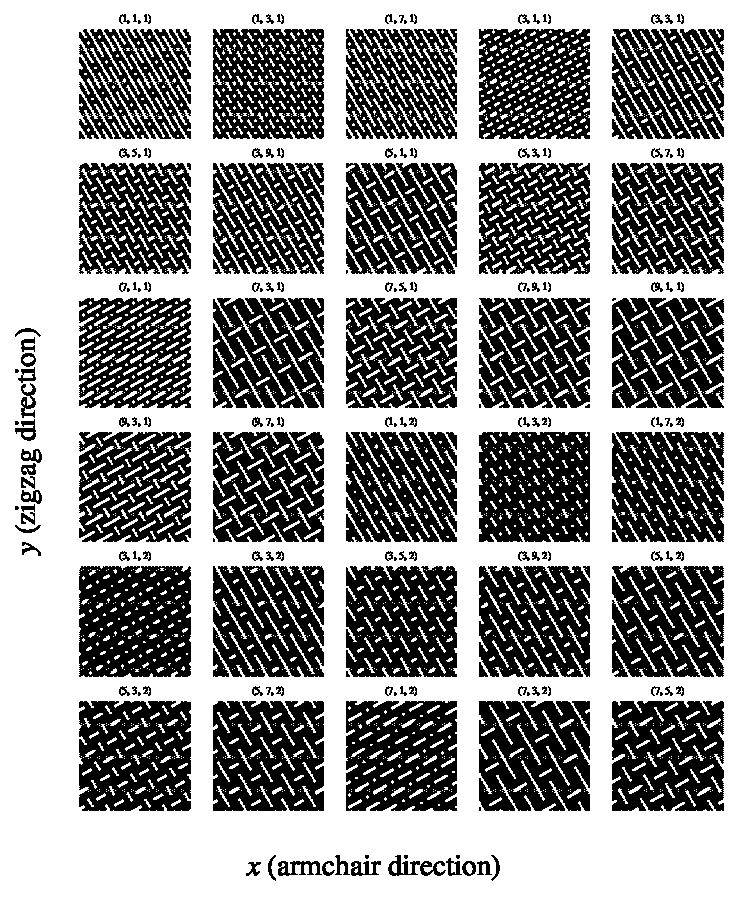
\includegraphics[width=\linewidth]{figures/dataset/popup_0.pdf}
    \caption{Tetrahedron patterns.}
    \label{fig:T0}
\end{figure}
\begin{figure}[H]
    \centering
    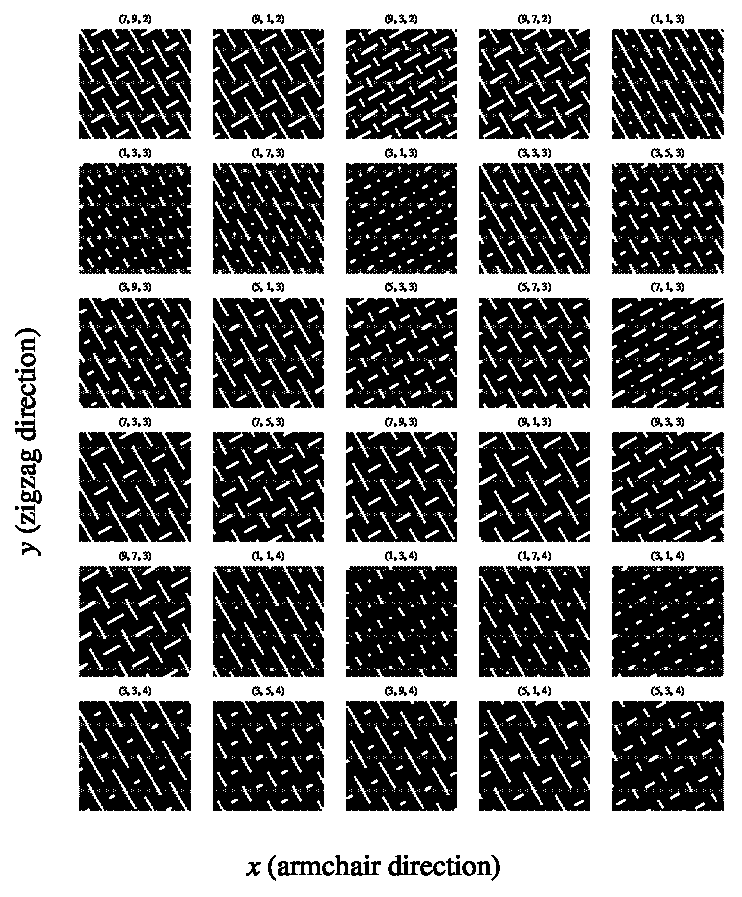
\includegraphics[width=\linewidth]{figures/dataset/popup_1.pdf}
    \caption{Tetrahedron patterns.}
    \label{fig:T1}
\end{figure}
\begin{figure}[H]
    \centering
    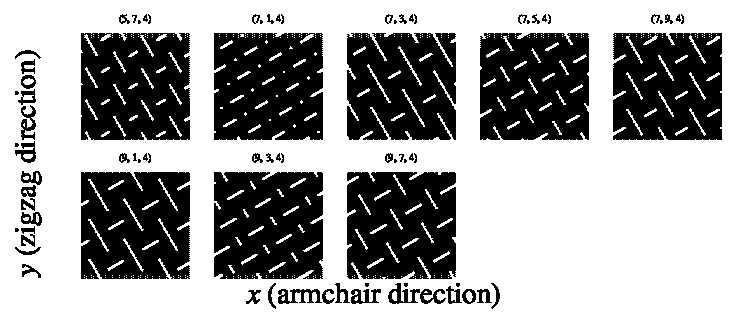
\includegraphics[width=\linewidth]{figures/dataset/popup_2.pdf}
    \caption{Tetrahedron patterns.}
    \label{fig:T2}
\end{figure}


\subsection{Honeycomb}
\begin{figure}[H]
    \centering
    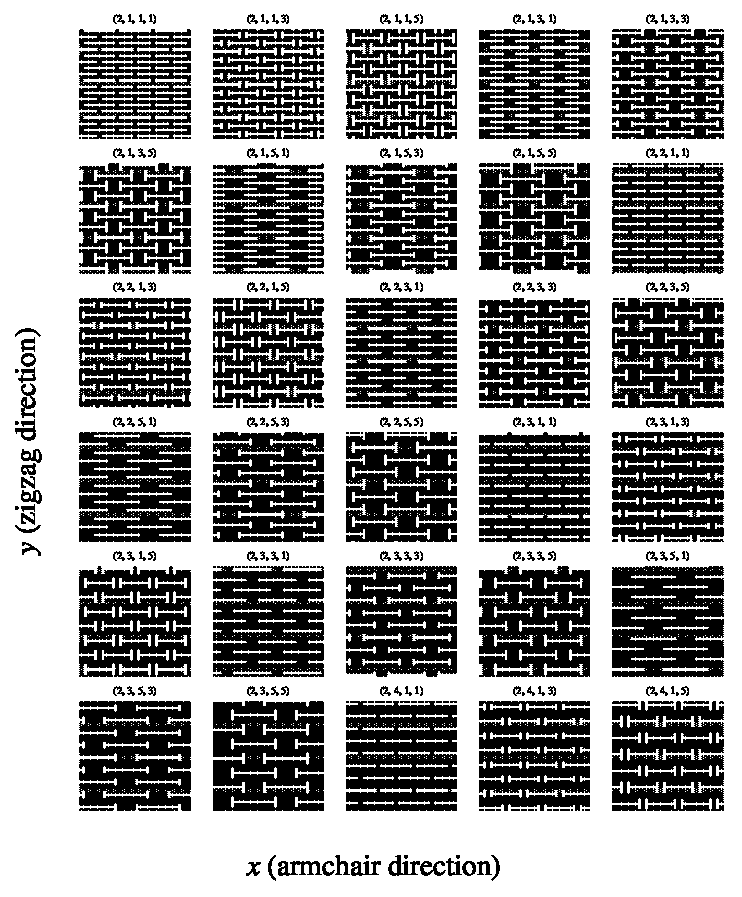
\includegraphics[width=\linewidth]{figures/dataset/honeycomb_0.pdf}
    \caption{Honeycomb patterns.}
    \label{fig:H0}
\end{figure}
\begin{figure}[H]
    \centering
    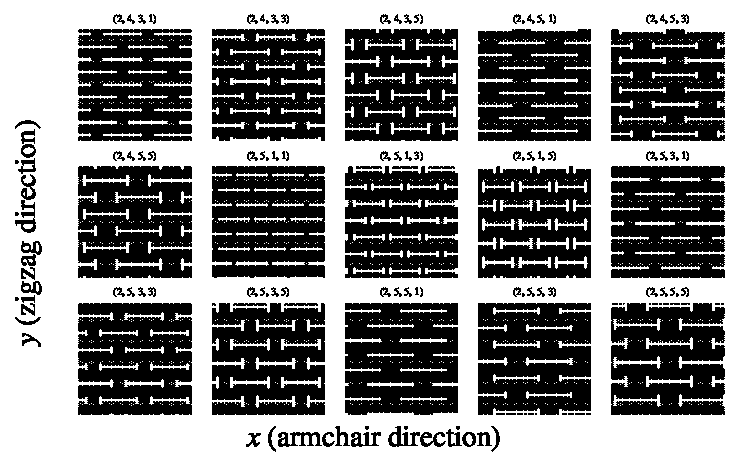
\includegraphics[width=\linewidth]{figures/dataset/honeycomb_1.pdf}
    \caption{Honeycomb patterns.}
    \label{fig:H1}
\end{figure}

\subsection{Random walk}
\begin{figure}[H]
    \centering
    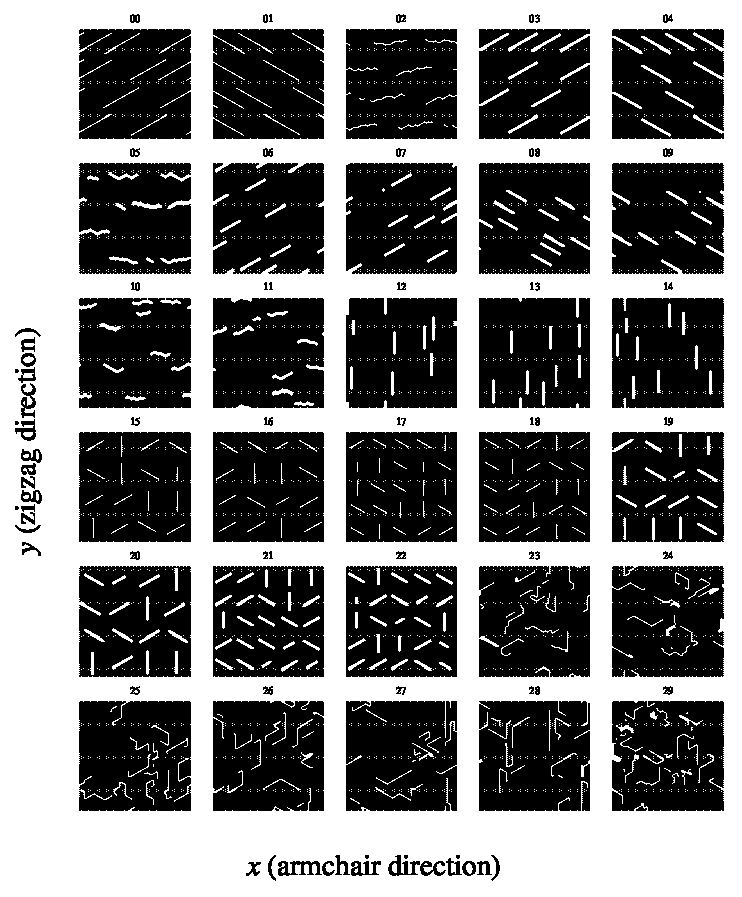
\includegraphics[width=\linewidth]{figures/dataset/RW_0.pdf}
    \caption{Random walk patterns.}
    \label{fig:R0}
\end{figure}
\begin{figure}[H]
    \centering
    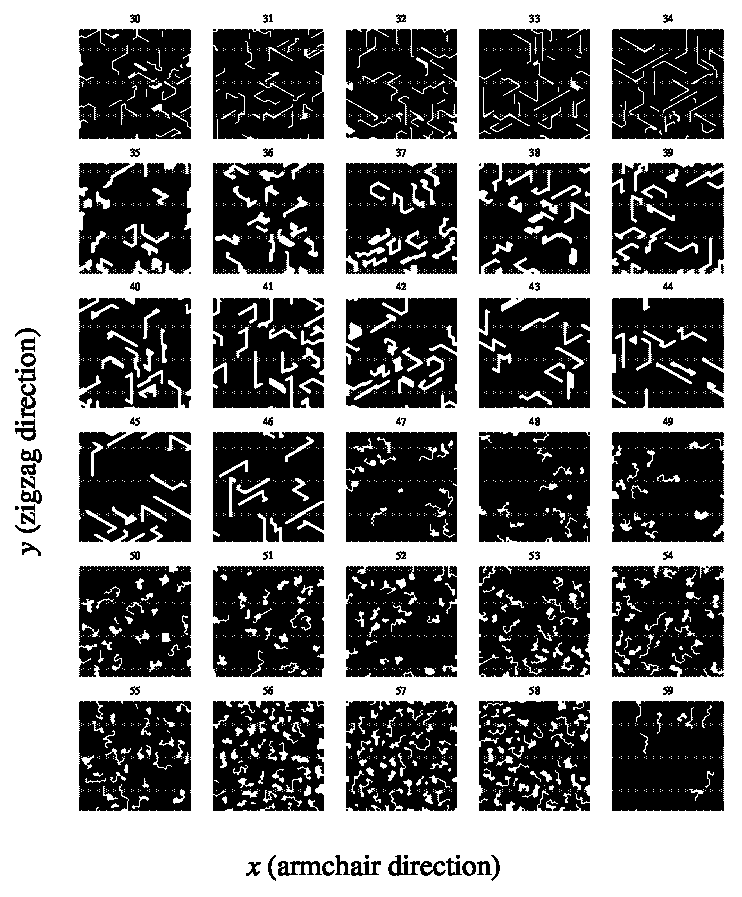
\includegraphics[width=\linewidth]{figures/dataset/RW_1.pdf}
    \caption{Random walk patterns.}
    \label{fig:R1}
\end{figure}
\begin{figure}[H]
    \centering
    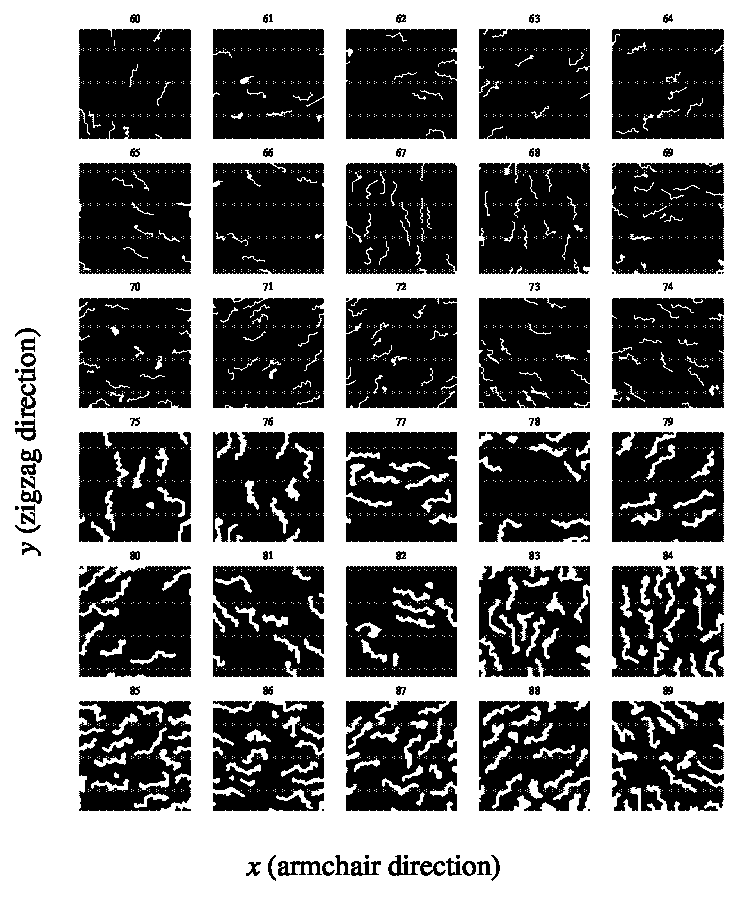
\includegraphics[width=\linewidth]{figures/dataset/RW_2.pdf}
    \caption{Random walk patterns.}
    \label{fig:R2}
\end{figure}
\begin{figure}[H]
    \centering
    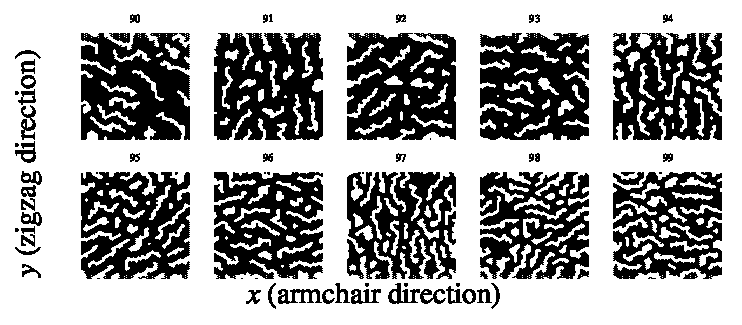
\includegraphics[width=\linewidth]{figures/dataset/RW_3.pdf}
    \caption{Random walk patterns.}
    \label{fig:R3}
\end{figure}


\newcolumntype{C}[1]{>{\centering\let\newline\\\arraybackslash\hspace{0pt}}m{#1}}
\begin{longtable}{|C{0.9cm}|C{0.8cm}|C{0.8cm}|C{0.8cm}|C{3cm}|C{1.5cm}|C{1.5cm}|C{0.8cm}|C{0.8cm}|C{1cm}|C{1cm}|} \hline
    Index & Num. \newline walks & Max. steps & Min. dis. & Bias \newline (dir., temp.) & Connection & Avoid unvalid & RN6 & Grid start & Centering & Stay or break  \ \\ \hline
    0 &  10 &  40 &  4 & (up right, 100) & Atom & False & False & True & True & 0 \\ \hline
    1 &  10 &  40 &  4 & (down right, 100) & Atom & False & False & True & True & 0 \\ \hline
    2 &  10 &  40 &  4 & (up, 100) & Atom & False & False & True & True & 0 \\ \hline
    3 &  10 &  15 &  4 & (up right, 100) & Center & False & False & True & True & 0 \\ \hline
    4 &  10 &  15 &  4 & (down right, 100) & Center & False & False & True & True & 0 \\ \hline
    5 &  10 &  15 &  4 & (up, 100) & Center & False & False & True & True & 0 \\ \hline


    6-7 &  10 &  10 &  4 & (up right, 100) & Center & False & False & False & False & 0 \\ \hline
    % 7 &  10 &  10 &  4 & (up right, 100) & Center & False & False & False & False & 0 \\ \hline

    8-9 &  10 &  10 &  4 & (down right, 100) & Center & False & False & False & False & 0 \\ \hline
    % 9 &  10 &  10 &  4 & (down right, 100) & Center & False & False & False & False & 0 \\ \hline

    10-11 &  10 &  10 &  4 & (up, 100) & Center & False & False & False & False & 0 \\ \hline
    % 11 &  10 &  10 &  4 & (up, 100) & Center & False & False & False & False & 0 \\ \hline

    12-14 &  10 &  10 &  4 & (right, 100) & Center & False & False & False & False & 0 \\ \hline
    % 13 &  10 &  10 &  4 & (right, 100) & Center & False & False & False & False & 0 \\ \hline
    % 14 &  10 &  10 &  4 & (right, 100) & Center & False & False & False & False & 0 \\ \hline

    15-16 &  16 &  20 &  3 & (None, 100) & Atom & False & True & True & True & 0 \\ \hline
    % 16 &  16 &  20 &  3 & (None, 100) & Atom & False & True & True & True & 0 \\ \hline

    17-18 &  25 &  15 &  3 & (None, 100) & Atom & False & True & True & True & 0 \\ \hline
    % 18 &  25 &  15 &  3 & (None, 100) & Atom & False & True & True & True & 0 \\ \hline

    19-20 &  16 &  10 &  3 & (None, 100) & Center & False & True & True & True & 0 \\ \hline
    % 20 &  16 &  10 &  3 & (None, 100) & Center & False & True & True & True & 0 \\ \hline

    21-22 &  25 &  8 &  3 & (None, 100) & Center & False & True & True & True & 0 \\ \hline
    % 22 &  25 &  8 &  3 & (None, 100) & Center & False & True & True & True & 0 \\ \hline

    23-24 &  15 &  40 &  3 & (None, 0) & Atom & True & True & False & False & 0.85 \\ \hline
    % 24 &  15 &  40 &  3 & (None, 0) & Atom & True & True & False & False & 0.85 \\ \hline

    25-26 &  15 &  40 &  3 & (None, 0) & Atom & True & True & False & False & 0.9 \\ \hline
    % 26 &  15 &  40 &  3 & (None, 0) & Atom & True & True & False & False & 0.9 \\ \hline

    27-28 &  15 &  40 &  3 & (None, 0) & Atom & True & True & False & False & 0.95 \\ \hline
    % 28 &  15 &  40 &  3 & (None, 0) & Atom & True & True & False & False & 0.95 \\ \hline

    29-30 &  25 &  40 &  3 & (None, 0) & Atom & True & True & False & False & 0.85 \\ \hline
    % 30 &  25 &  40 &  3 & (None, 0) & Atom & True & True & False & False & 0.85 \\ \hline

    31-32 &  25 &  40 &  3 & (None, 0) & Atom & True & True & False & False & 0.9 \\ \hline
    % 32 &  25 &  40 &  3 & (None, 0) & Atom & True & True & False & False & 0.9 \\ \hline

    33-34 &  25 &  40 &  3 & (None, 0) & Atom & True & True & False & False & 0.95 \\ \hline
    % 34 &  25 &  40 &  3 & (None, 0) & Atom & True & True & False & False & 0.95 \\ \hline
    
    35-38 &  15 &  20 &  3 & (None, 0) & Center & True & True & False & False & 0.7 \\ \hline
    % 36 &  15 &  20 &  3 & (None, 0) & Center & True & True & False & False & 0.7 \\ \hline
    % 37 &  15 &  20 &  3 & (None, 0) & Center & True & True & False & False & 0.7 \\ \hline
    % 38 &  15 &  20 &  3 & (None, 0) & Center & True & True & False & False & 0.7 \\ \hline

    39-42 &  15 &  20 &  3 & (None, 0) & Center & True & True & False & False & 0.8 \\ \hline
    % 40 &  15 &  20 &  3 & (None, 0) & Center & True & True & False & False & 0.8 \\ \hline
    % 41 &  15 &  20 &  3 & (None, 0) & Center & True & True & False & False & 0.8 \\ \hline
    % 42 &  15 &  20 &  3 & (None, 0) & Center & True & True & False & False & 0.8 \\ \hline

    43-46 &  10 &  20 &  3 & (None, 0) & Center & True & True & False & False & 0.9 \\ \hline
    % 44 &  10 &  20 &  3 & (None, 0) & Center & True & True & False & False & 0.9 \\ \hline
    % 45 &  10 &  20 &  3 & (None, 0) & Center & True & True & False & False & 0.9 \\ \hline
    % 46 &  10 &  20 &  3 & (None, 0) & Center & True & True & False & False & 0.9 \\ \hline
    
    
    47-49 &  15 &  40 &  4 & (None, 0) & Atom & True & False & False & False & 0 \\ \hline
    % 48 &  15 &  40 &  4 & (None, 0) & Atom & True & False & False & False & 0 \\ \hline
    % 49 &  15 &  40 &  4 & (None, 0) & Atom & True & False & False & False & 0 \\ \hline

    50-52 &  25 &  40 &  4 & (None, 0) & Atom & True & False & False & False & 0 \\ \hline
    % 51 &  25 &  40 &  4 & (None, 0) & Atom & True & False & False & False & 0 \\ \hline
    % 52 &  25 &  40 &  4 & (None, 0) & Atom & True & False & False & False & 0 \\ \hline

    53-55 &  30 &  40 &  4 & (None, 0) & Atom & True & False & False & False & 0 \\ \hline
    % 54 &  30 &  40 &  4 & (None, 0) & Atom & True & False & False & False & 0 \\ \hline
    % 55 &  30 &  40 &  4 & (None, 0) & Atom & True & False & False & False & 0 \\ \hline

    56-58 &  50 &  40 &  4 & (None, 0) & Atom & True & False & False & False & 0 \\ \hline
    % 57 &  50 &  40 &  4 & (None, 0) & Atom & True & False & False & False & 0 \\ \hline
    % 58 &  50 &  40 &  4 & (None, 0) & Atom & True & False & False & False & 0 \\ \hline
    
    
    59-60 &  8 &  30 &  4 & (right, 1) & Atom & True & False & False & False & 0 \\ \hline
    % 60 &  8 &  30 &  4 & (right, 1) & Atom & True & False & False & False & 0 \\ \hline

    61-62 &  8 &  30 &  4 & (up, 1) & Atom & True & False & False & False & 0 \\ \hline
    % 62 &  8 &  30 &  4 & (up, 1) & Atom & True & False & False & False & 0 \\ \hline

    63-64 &  8 &  30 &  4 & (up right, 1) & Atom & True & False & False & False & 0 \\ \hline
    % 64 &  8 &  30 &  4 & (up right, 1) & Atom & True & False & False & False & 0 \\ \hline

    65-66 &  8 &  30 &  4 & (down right, 1) & Atom & True & False & False & False & 0 \\ \hline
    % 66 &  8 &  30 &  4 & (down right, 1) & Atom & True & False & False & False & 0 \\ \hline

    67-68 &  16 &  30 &  4 & (right, 1) & Atom & True & False & False & False & 0 \\ \hline
    % 68 &  16 &  30 &  4 & (right, 1) & Atom & True & False & False & False & 0 \\ \hline

    69-70 &  16 &  30 &  4 & (up, 1) & Atom & True & False & False & False & 0 \\ \hline
    % 70 &  16 &  30 &  4 & (up, 1) & Atom & True & False & False & False & 0 \\ \hline

    71-72 &  16 &  30 &  4 & (up right, 1) & Atom & True & False & False & False & 0 \\ \hline
    % 72 &  16 &  30 &  4 & (up right, 1) & Atom & True & False & False & False & 0 \\ \hline

    73-74 &  16 &  30 &  4 & (down right, 1) & Atom & True & False & False & False & 0 \\ \hline
    % 74 &  16 &  30 &  4 & (down right, 1) & Atom & True & False & False & False & 0 \\ \hline
    
    
    75-76 &  8 &  30 &  4 & (right, 1) & Center & True & False & False & False & 0 \\ \hline
    % 76 &  8 &  30 &  4 & (right, 1) & Center & True & False & False & False & 0 \\ \hline

    77-78 &  8 &  30 &  4 & (up, 1) & Center & True & False & False & False & 0 \\ \hline
    % 78 &  8 &  30 &  4 & (up, 1) & Center & True & False & False & False & 0 \\ \hline

    79-78 &  8 &  30 &  4 & (up right, 1) & Center & True & False & False & False & 0 \\ \hline
    % 80 &  8 &  30 &  4 & (up right, 1) & Center & True & False & False & False & 0 \\ \hline

    81-82 &  8 &  30 &  4 & (down right, 1) & Center & True & False & False & False & 0 \\ \hline
    % 82 &  8 &  30 &  4 & (down right, 1) & Center & True & False & False & False & 0 \\ \hline

    83-84 &  16 &  30 &  4 & (right, 1) & Center & True & False & False & False & 0 \\ \hline
    % 84 &  16 &  30 &  4 & (right, 1) & Center & True & False & False & False & 0 \\ \hline

    85-86 &  16 &  30 &  4 & (up, 1) & Center & True & False & False & False & 0 \\ \hline
    % 86 &  16 &  30 &  4 & (up, 1) & Center & True & False & False & False & 0 \\ \hline

    87-88 &  16 &  30 &  4 & (up right, 1) & Center & True & False & False & False & 0 \\ \hline
    % 88 &  16 &  30 &  4 & (up right, 1) & Center & True & False & False & False & 0 \\ \hline

    89-90 &  16 &  30 &  4 & (down right, 1) & Center & True & False & False & False & 0 \\ \hline
    % 90 &  16 &  30 &  4 & (down right, 1) & Center & True & False & False & False & 0 \\ \hline
    
    
    91 &  32 &  30 &  5 & (down, 1.2) & Center & True & False & False & False & 0 \\ \hline

    92 &  32 &  30 &  5 & (down left, 1.2) & Center & True & False & False & False & 0 \\ \hline

    93 &  32 &  30 &  5 & (left, 1.2) & Center & True & False & False & False & 0 \\ \hline

    94 &  32 &  30 &  4 & (down, 1.2) & Center & True & False & False & False & 0 \\ \hline

    95 &  32 &  30 &  4 & (down left, 1.2) & Center & True & False & False & False & 0 \\ \hline

    96 &  32 &  30 &  4 & (left, 1.2) & Center & True & False & False & False & 0 \\ \hline

    97 &  32 &  30 &  3 & (down, 1.2) & Center & True & False & False & False & 0 \\ \hline

    98 &  32 &  30 &  3 & (down left, 1.2) & Center & True & False & False & False & 0 \\ \hline

    99 &  32 &  30 &  3 & (left, 1.2) & Center & True & False & False & False & 0 \\ \hline
    \caption{Random walk parameters corresponidng to the configurations shown in figure \ref{fig:R0}-\ref{fig:R3}. All configurations have the default parameters: Periodic = True, Avoid clustering = 10}
    \label{tab:RW_details}
    \end{longtable}

% \begin{table}[H]
%     \begin{center}
%     \caption{Settings for random walk. Default: Periodic = True, Avoid cluster = ?}
%     \label{tab:dataset_summary}
%     \begin{tabular}{|C{0.9cm}|C{0.8cm}|C{0.8cm}|C{0.8cm}|C{3cm}|C{1.5cm}|C{1.5cm}|C{0.7cm}|C{0.8cm}|C{1cm}|C{1cm}|} \hline
%     Index & Num. \newline walks & Max. steps & Min. dis. & Bias (dir, temp) & Connection & Avoid unvalid & RN6 & Grid start & Centering & Stay or break  \ \\ \hline
%     0 &  10 &  40 &  4 & (up right, 100) & False & False & False & True & True & 0 \\ \hline
%     1 &  10 &  40 &  4 & (down right, 100) & False & False & False & True & True & 0 \\ \hline
%     2 &  10 &  40 &  4 & (up, 100) & False & False & False & True & True & 0 \\ \hline
%     3 &  10 &  15 &  4 & (up right, 100) & True & False & False & True & True & 0 \\ \hline
%     4 &  10 &  15 &  4 & (down right, 100) & True & False & False & True & True & 0 \\ \hline
%     5 &  10 &  15 &  4 & (up, 100) & True & False & False & True & True & 0 \\ \hline


%     6-7 &  10 &  10 &  4 & (up right, 100) & True & False & False & False & False & 0 \\ \hline
%     % 7 &  10 &  10 &  4 & (up right, 100) & True & False & False & False & False & 0 \\ \hline

%     8-9 &  10 &  10 &  4 & (down right, 100) & True & False & False & False & False & 0 \\ \hline
%     % 9 &  10 &  10 &  4 & (down right, 100) & True & False & False & False & False & 0 \\ \hline

%     10-11 &  10 &  10 &  4 & (up, 100) & True & False & False & False & False & 0 \\ \hline
%     % 11 &  10 &  10 &  4 & (up, 100) & True & False & False & False & False & 0 \\ \hline

%     12-14 &  10 &  10 &  4 & (right, 100) & True & False & False & False & False & 0 \\ \hline
%     % 13 &  10 &  10 &  4 & (right, 100) & True & False & False & False & False & 0 \\ \hline
%     % 14 &  10 &  10 &  4 & (right, 100) & True & False & False & False & False & 0 \\ \hline

%     15-16 &  16 &  20 &  3 & (None, 100) & False & False & True & True & True & 0 \\ \hline
%     % 16 &  16 &  20 &  3 & (None, 100) & False & False & True & True & True & 0 \\ \hline

%     17-18 &  25 &  15 &  3 & (None, 100) & False & False & True & True & True & 0 \\ \hline
%     % 18 &  25 &  15 &  3 & (None, 100) & False & False & True & True & True & 0 \\ \hline

%     19-20 &  16 &  10 &  3 & (None, 100) & True & False & True & True & True & 0 \\ \hline
%     % 20 &  16 &  10 &  3 & (None, 100) & True & False & True & True & True & 0 \\ \hline

%     21-22 &  25 &  8 &  3 & (None, 100) & True & False & True & True & True & 0 \\ \hline
%     % 22 &  25 &  8 &  3 & (None, 100) & True & False & True & True & True & 0 \\ \hline

%     23-24 &  15 &  40 &  3 & (None, 0) & False & True & True & False & False & 0.85 \\ \hline
%     % 24 &  15 &  40 &  3 & (None, 0) & False & True & True & False & False & 0.85 \\ \hline

%     25-26 &  15 &  40 &  3 & (None, 0) & False & True & True & False & False & 0.9 \\ \hline
%     % 26 &  15 &  40 &  3 & (None, 0) & False & True & True & False & False & 0.9 \\ \hline

%     27-28 &  15 &  40 &  3 & (None, 0) & False & True & True & False & False & 0.95 \\ \hline
%     % 28 &  15 &  40 &  3 & (None, 0) & False & True & True & False & False & 0.95 \\ \hline

%     29-30 &  25 &  40 &  3 & (None, 0) & False & True & True & False & False & 0.85 \\ \hline
%     % 30 &  25 &  40 &  3 & (None, 0) & False & True & True & False & False & 0.85 \\ \hline

%     31-32 &  25 &  40 &  3 & (None, 0) & False & True & True & False & False & 0.9 \\ \hline
%     % 32 &  25 &  40 &  3 & (None, 0) & False & True & True & False & False & 0.9 \\ \hline

%     33-34 &  25 &  40 &  3 & (None, 0) & False & True & True & False & False & 0.95 \\ \hline
%     % 34 &  25 &  40 &  3 & (None, 0) & False & True & True & False & False & 0.95 \\ \hline
    
%     35-38 &  15 &  20 &  3 & (None, 0) & True & True & True & False & False & 0.7 \\ \hline
%     % 36 &  15 &  20 &  3 & (None, 0) & True & True & True & False & False & 0.7 \\ \hline
%     % 37 &  15 &  20 &  3 & (None, 0) & True & True & True & False & False & 0.7 \\ \hline
%     % 38 &  15 &  20 &  3 & (None, 0) & True & True & True & False & False & 0.7 \\ \hline

%     39-42 &  15 &  20 &  3 & (None, 0) & True & True & True & False & False & 0.8 \\ \hline
%     % 40 &  15 &  20 &  3 & (None, 0) & True & True & True & False & False & 0.8 \\ \hline
%     % 41 &  15 &  20 &  3 & (None, 0) & True & True & True & False & False & 0.8 \\ \hline
%     % 42 &  15 &  20 &  3 & (None, 0) & True & True & True & False & False & 0.8 \\ \hline

%     43-46 &  10 &  20 &  3 & (None, 0) & True & True & True & False & False & 0.9 \\ \hline
%     % 44 &  10 &  20 &  3 & (None, 0) & True & True & True & False & False & 0.9 \\ \hline
%     % 45 &  10 &  20 &  3 & (None, 0) & True & True & True & False & False & 0.9 \\ \hline
%     % 46 &  10 &  20 &  3 & (None, 0) & True & True & True & False & False & 0.9 \\ \hline
    
    
%     47-49 &  15 &  40 &  4 & (None, 0) & False & True & False & False & False & 0 \\ \hline
%     % 48 &  15 &  40 &  4 & (None, 0) & False & True & False & False & False & 0 \\ \hline
%     % 49 &  15 &  40 &  4 & (None, 0) & False & True & False & False & False & 0 \\ \hline

%     50-52 &  25 &  40 &  4 & (None, 0) & False & True & False & False & False & 0 \\ \hline
%     % 51 &  25 &  40 &  4 & (None, 0) & False & True & False & False & False & 0 \\ \hline
%     % 52 &  25 &  40 &  4 & (None, 0) & False & True & False & False & False & 0 \\ \hline

%     53-55 &  30 &  40 &  4 & (None, 0) & False & True & False & False & False & 0 \\ \hline
%     % 54 &  30 &  40 &  4 & (None, 0) & False & True & False & False & False & 0 \\ \hline
%     % 55 &  30 &  40 &  4 & (None, 0) & False & True & False & False & False & 0 \\ \hline

%     56-58 &  50 &  40 &  4 & (None, 0) & False & True & False & False & False & 0 \\ \hline
%     % 57 &  50 &  40 &  4 & (None, 0) & False & True & False & False & False & 0 \\ \hline
%     % 58 &  50 &  40 &  4 & (None, 0) & False & True & False & False & False & 0 \\ \hline
    
    
%     59-60 &  8 &  30 &  4 & (right, 1) & False & True & False & False & False & 0 \\ \hline
%     % 60 &  8 &  30 &  4 & (right, 1) & False & True & False & False & False & 0 \\ \hline

%     61-62 &  8 &  30 &  4 & (up, 1) & False & True & False & False & False & 0 \\ \hline
%     % 62 &  8 &  30 &  4 & (up, 1) & False & True & False & False & False & 0 \\ \hline

%     63-64 &  8 &  30 &  4 & (up right, 1) & False & True & False & False & False & 0 \\ \hline
%     % 64 &  8 &  30 &  4 & (up right, 1) & False & True & False & False & False & 0 \\ \hline

%     65-66 &  8 &  30 &  4 & (down right, 1) & False & True & False & False & False & 0 \\ \hline
%     % 66 &  8 &  30 &  4 & (down right, 1) & False & True & False & False & False & 0 \\ \hline

%     67-68 &  16 &  30 &  4 & (right, 1) & False & True & False & False & False & 0 \\ \hline
%     % 68 &  16 &  30 &  4 & (right, 1) & False & True & False & False & False & 0 \\ \hline

%     69-70 &  16 &  30 &  4 & (up, 1) & False & True & False & False & False & 0 \\ \hline
%     % 70 &  16 &  30 &  4 & (up, 1) & False & True & False & False & False & 0 \\ \hline

%     71-72 &  16 &  30 &  4 & (up right, 1) & False & True & False & False & False & 0 \\ \hline
%     % 72 &  16 &  30 &  4 & (up right, 1) & False & True & False & False & False & 0 \\ \hline

%     73-74 &  16 &  30 &  4 & (down right, 1) & False & True & False & False & False & 0 \\ \hline
%     % 74 &  16 &  30 &  4 & (down right, 1) & False & True & False & False & False & 0 \\ \hline
    
    
%     75-76 &  8 &  30 &  4 & (right, 1) & True & True & False & False & False & 0 \\ \hline
%     % 76 &  8 &  30 &  4 & (right, 1) & True & True & False & False & False & 0 \\ \hline

%     77-78 &  8 &  30 &  4 & (up, 1) & True & True & False & False & False & 0 \\ \hline
%     % 78 &  8 &  30 &  4 & (up, 1) & True & True & False & False & False & 0 \\ \hline

%     79-78 &  8 &  30 &  4 & (up right, 1) & True & True & False & False & False & 0 \\ \hline
%     % 80 &  8 &  30 &  4 & (up right, 1) & True & True & False & False & False & 0 \\ \hline

%     81-82 &  8 &  30 &  4 & (down right, 1) & True & True & False & False & False & 0 \\ \hline
%     % 82 &  8 &  30 &  4 & (down right, 1) & True & True & False & False & False & 0 \\ \hline

%     83-84 &  16 &  30 &  4 & (right, 1) & True & True & False & False & False & 0 \\ \hline
%     % 84 &  16 &  30 &  4 & (right, 1) & True & True & False & False & False & 0 \\ \hline

%     85-86 &  16 &  30 &  4 & (up, 1) & True & True & False & False & False & 0 \\ \hline
%     % 86 &  16 &  30 &  4 & (up, 1) & True & True & False & False & False & 0 \\ \hline

%     87-88 &  16 &  30 &  4 & (up right, 1) & True & True & False & False & False & 0 \\ \hline
%     % 88 &  16 &  30 &  4 & (up right, 1) & True & True & False & False & False & 0 \\ \hline

%     89-90 &  16 &  30 &  4 & (down right, 1) & True & True & False & False & False & 0 \\ \hline
%     % 90 &  16 &  30 &  4 & (down right, 1) & True & True & False & False & False & 0 \\ \hline
    
    
%     91 &  32 &  30 &  5 & (down, 1.2) & True & True & False & False & False & 0 \\ \hline

%     92 &  32 &  30 &  5 & (down left, 1.2) & True & True & False & False & False & 0 \\ \hline

%     93 &  32 &  30 &  5 & (left, 1.2) & True & True & False & False & False & 0 \\ \hline

%     94 &  32 &  30 &  4 & (down, 1.2) & True & True & False & False & False & 0 \\ \hline

%     95 &  32 &  30 &  4 & (down left, 1.2) & True & True & False & False & False & 0 \\ \hline

%     96 &  32 &  30 &  4 & (left, 1.2) & True & True & False & False & False & 0 \\ \hline

%     97 &  32 &  30 &  3 & (down, 1.2) & True & True & False & False & False & 0 \\ \hline

%     98 &  32 &  30 &  3 & (down left, 1.2) & True & True & False & False & False & 0 \\ \hline

%     99 &  32 &  30 &  3 & (left, 1.2) & True & True & False & False & False & 0 \\ \hline
%     \end{tabular}
%     \end{center}
%   \end{table}



  
  

